\documentclass[11pt]{article}
\usepackage{amsmath,amssymb,amsthm}
\usepackage{graphicx}
\usepackage[margin=1in]{geometry}
\usepackage{fancyhdr}
\setlength{\parindent}{0pt}
\setlength{\parskip}{5pt plus 1pt}
\setlength{\headheight}{13.6pt}
\newcommand\question[2]{\vspace{.25in}\hrule\textbf{#1: #2}\vspace{.5em}\hrule\vspace{.10in}}
\renewcommand\part[1]{\vspace{.10in}\textbf{(#1)}}
\newcommand\algorithm{\vspace{.10in}\textbf{Algorithm: }}
\newcommand\correctness{\vspace{.10in}\textbf{Correctness: }}
\newcommand\runtime{\vspace{.10in}\textbf{Running time: }}
\pagestyle{fancyplain}
\lhead{\textbf{\NAME\ (\ANDREWID)}}
\chead{\textbf{HW\HWNUM}}
\rhead{02-713, \today}
\begin{document}\raggedright
	\newcommand\NAME{Muhammed Burak Bugrul}
	\newcommand\ANDREWID{150140015}
	\newcommand\HWNUM{1} 
    \question{Code}{}
        \textbf{draw(x, y, col, column)}: Draws a plot with input 'x', output 'y', color 'col' into 'column' subplot.\\
        \
        \\
        \textbf{standard\_deviation(x)}: Returns standard derivative of list 'x'.\\
        \
        \\
        \textbf{standard\_normalize(x)}: Performs standard normalization on list 'x' and returns a new list.\\
        \
        \\
        \textbf{convolution(a, b)}: Return convolution of 'a' and 'b'.\\
        \cleardoublepage
	\question{1. Signal}{}
    \part{functionA}
    \begin{figure}[h]
        \centering
        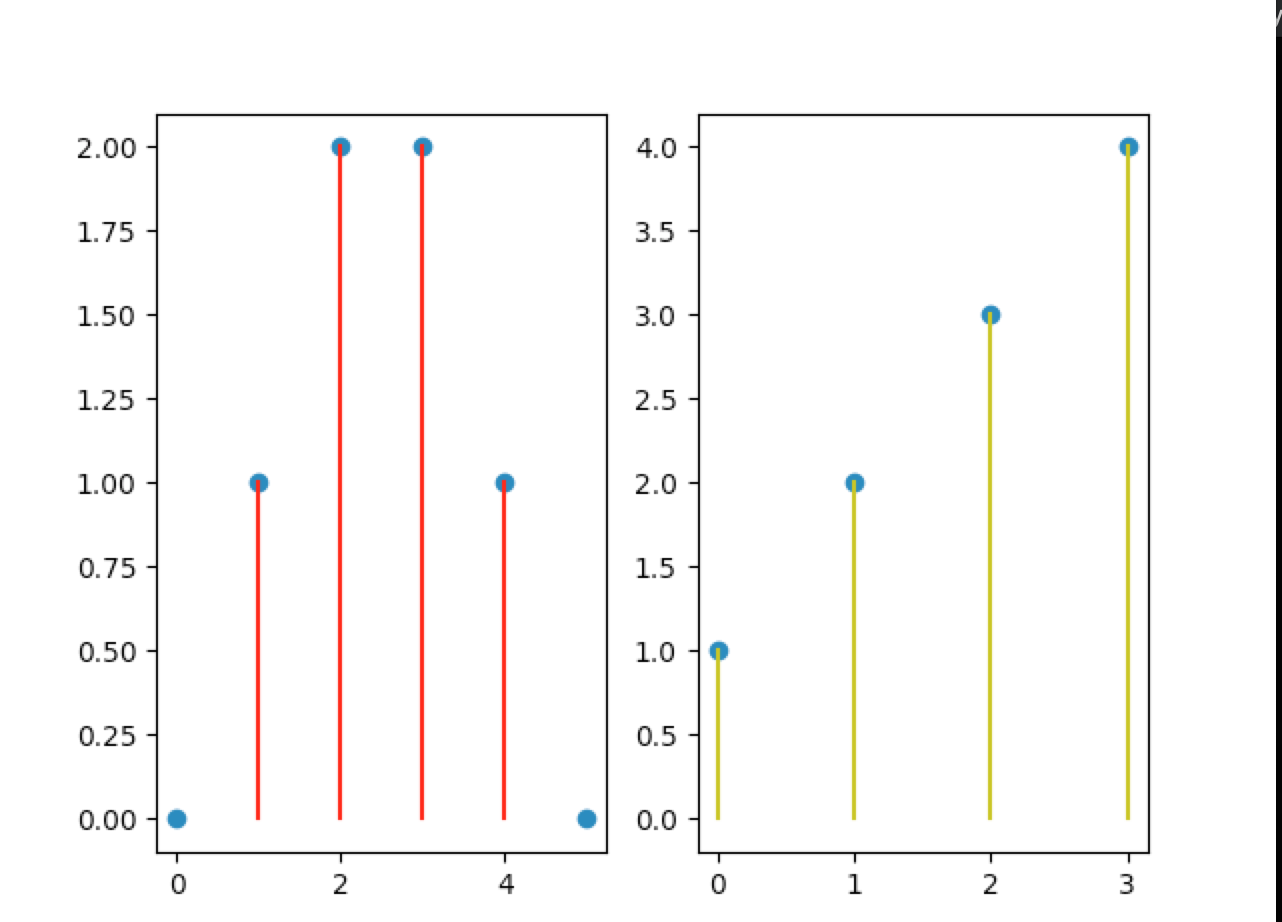
\includegraphics[width=0.5\linewidth]{figures/1a.png}
        \label{fig:1a}
    \end{figure}\\
    \part{functionB}
    \begin{figure}[h]
        \centering
        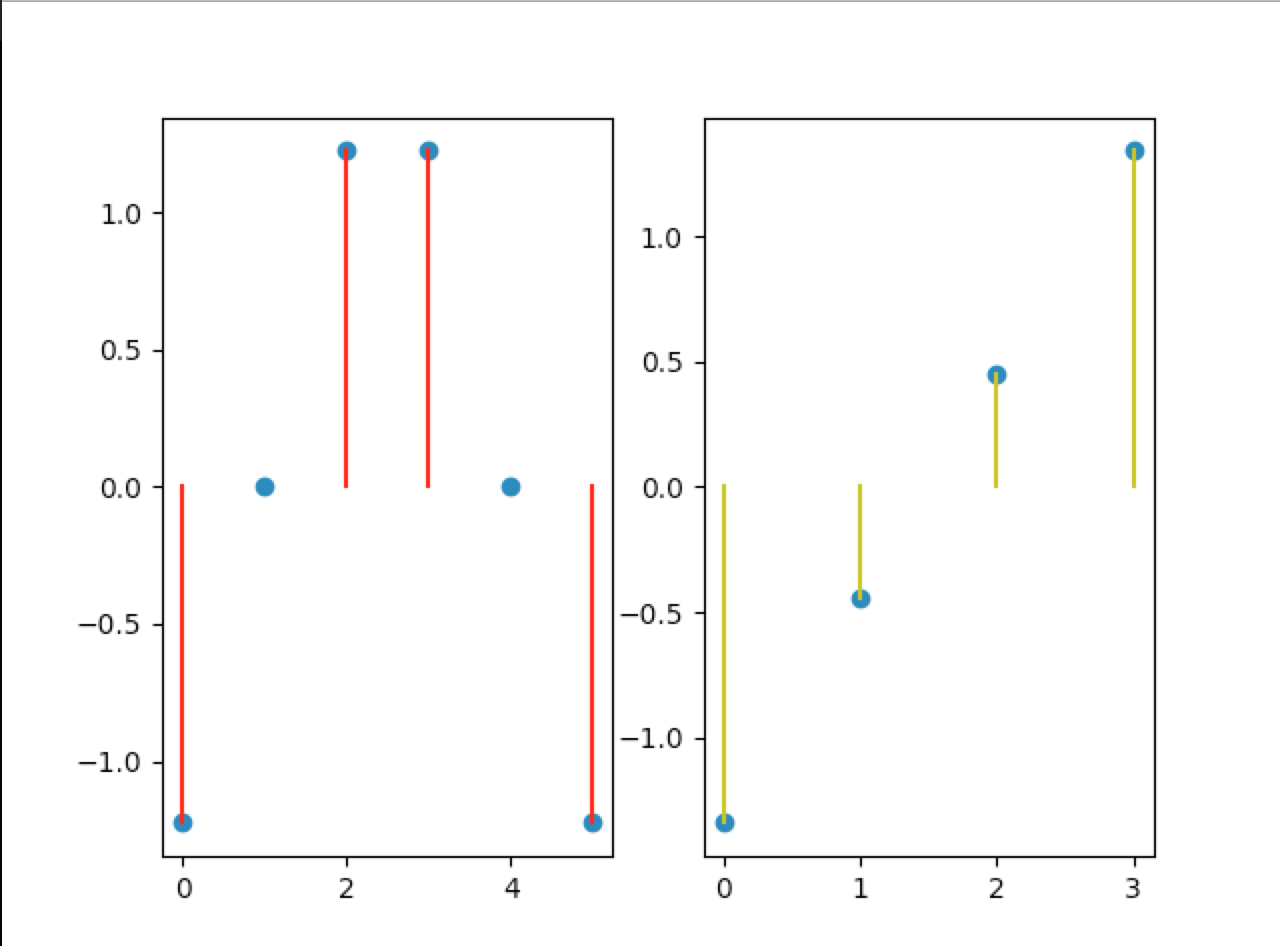
\includegraphics[width=0.5\linewidth]{figures/1b.png}
        \label{fig:1b}
    \end{figure}\\
    \part{functionC} [0, 1, 4, 9, 15, 16, 11, 4, 0]\\
     \part{functionD} [1.6431676725154982, 0.5477225575051661, -2.1908902300206643, -3.8340579025361627, 0.0, 3.8340579025361627, 2.1908902300206643, -0.5477225575051661, -1.6431676725154982]\\
     \cleardoublepage
     
     \question{2. Signal}{}
     \part{functionA}
     \begin{figure}[h]
         \centering
         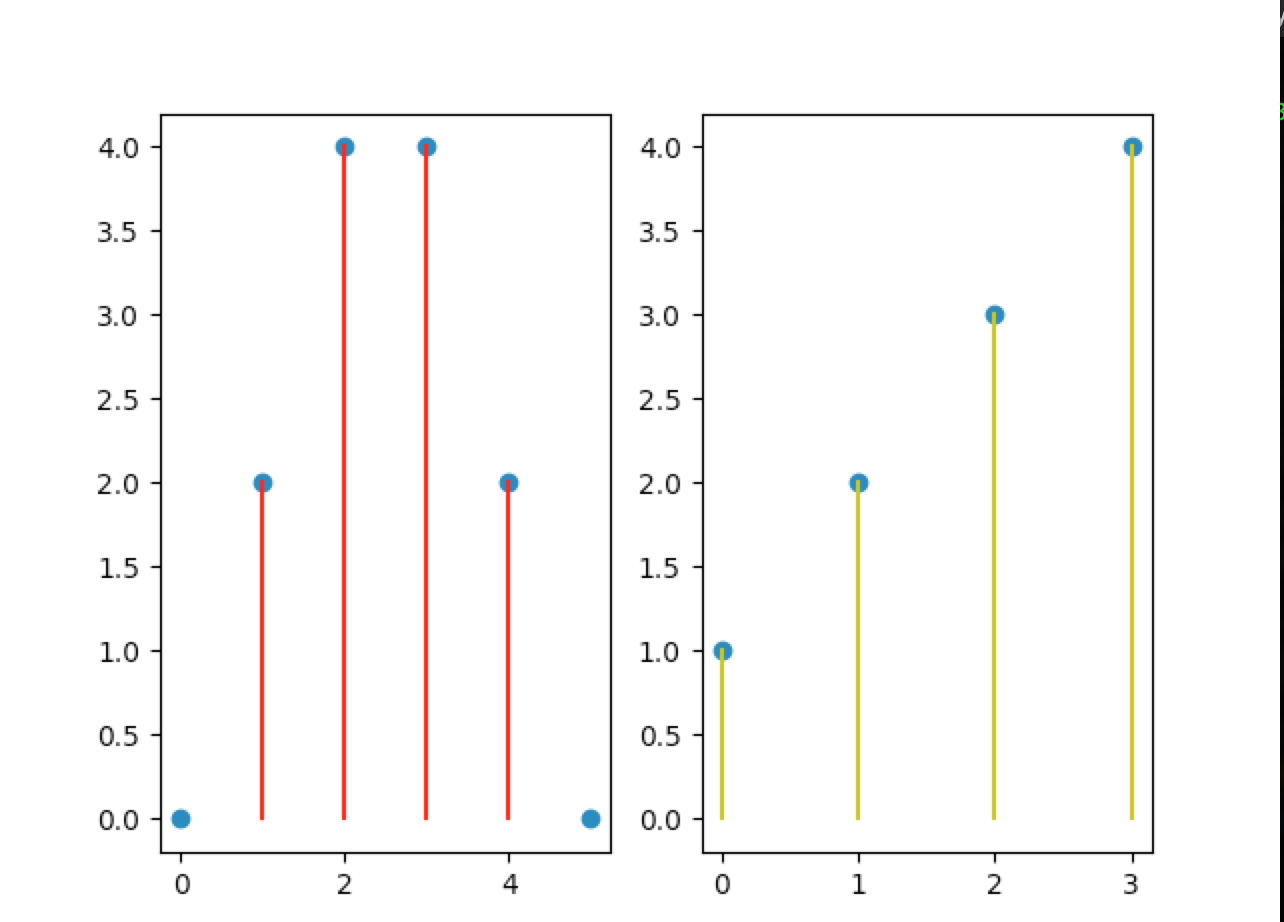
\includegraphics[width=0.5\linewidth]{figures/2a.png}
         \label{fig:2a}
     \end{figure}\\
     \part{functionB}
     \begin{figure}[h]
         \centering
         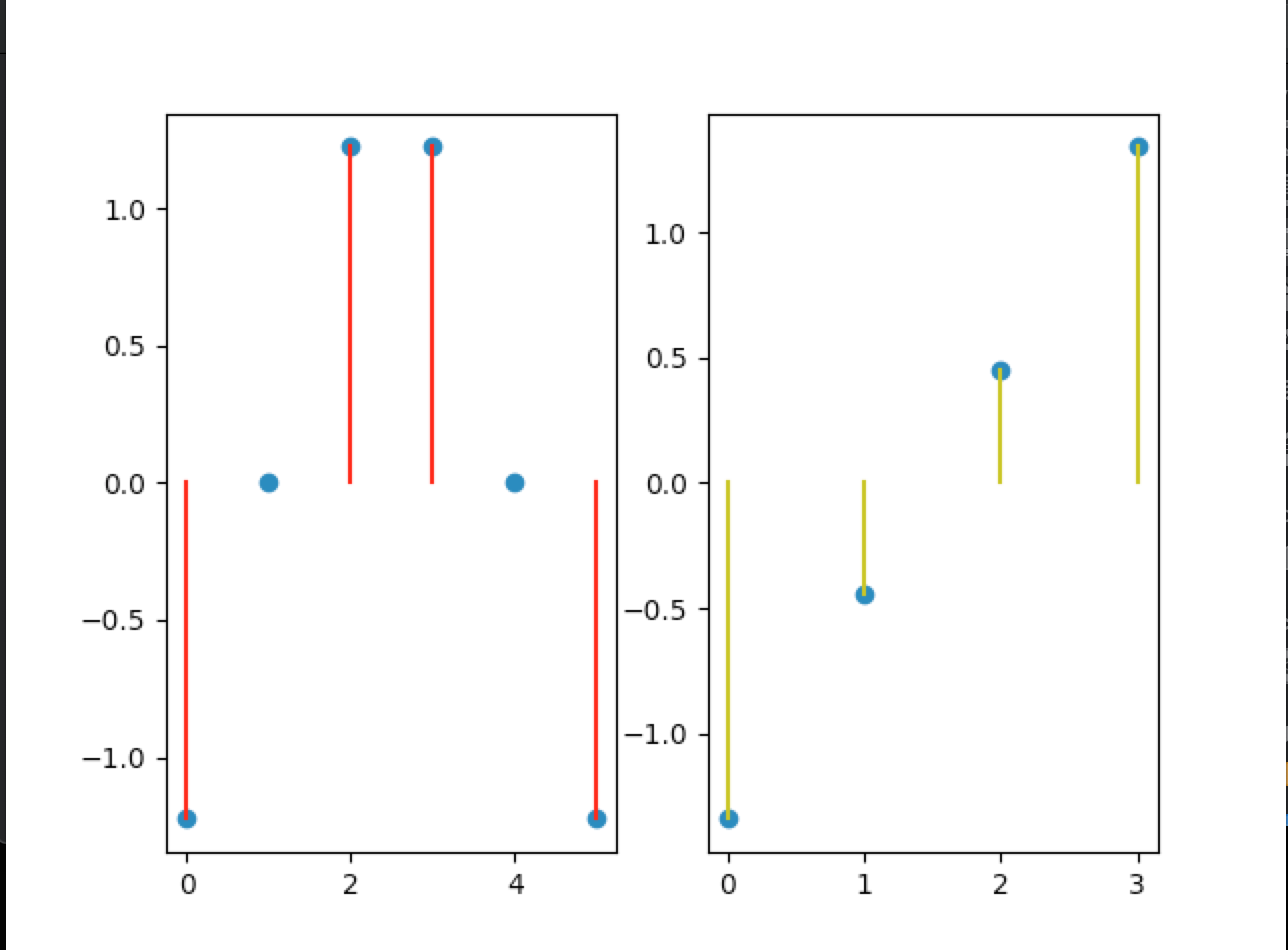
\includegraphics[width=0.5\linewidth]{figures/2b.png}
         \label{fig:2b}
     \end{figure}\\
     \part{functionC} [0, 2, 8, 18, 30, 32, 22, 8, 0]\\
     \part{functionD} [1.6431676725154982, 0.5477225575051661, -2.1908902300206643, -3.8340579025361627, 0.0, 3.8340579025361627, 2.1908902300206643, -0.5477225575051661, -1.6431676725154982]\\
     \cleardoublepage
     
      \question{3. Signal}{}
     \part{functionA}
     \begin{figure}[h]
         \centering
         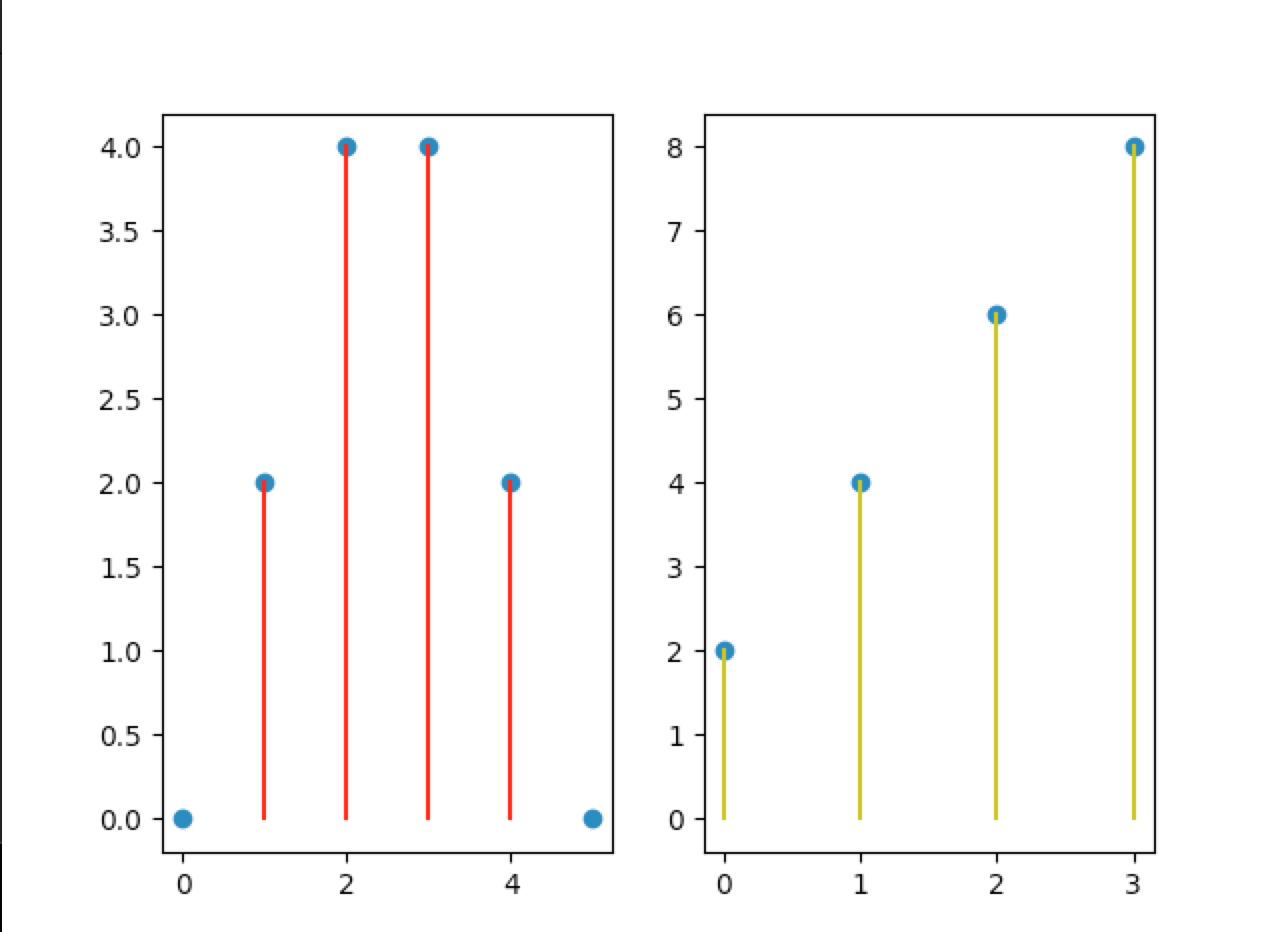
\includegraphics[width=0.5\linewidth]{figures/3a.png}
         \label{fig:3a}
     \end{figure}\\
     \part{functionB}
     \begin{figure}[h]
         \centering
         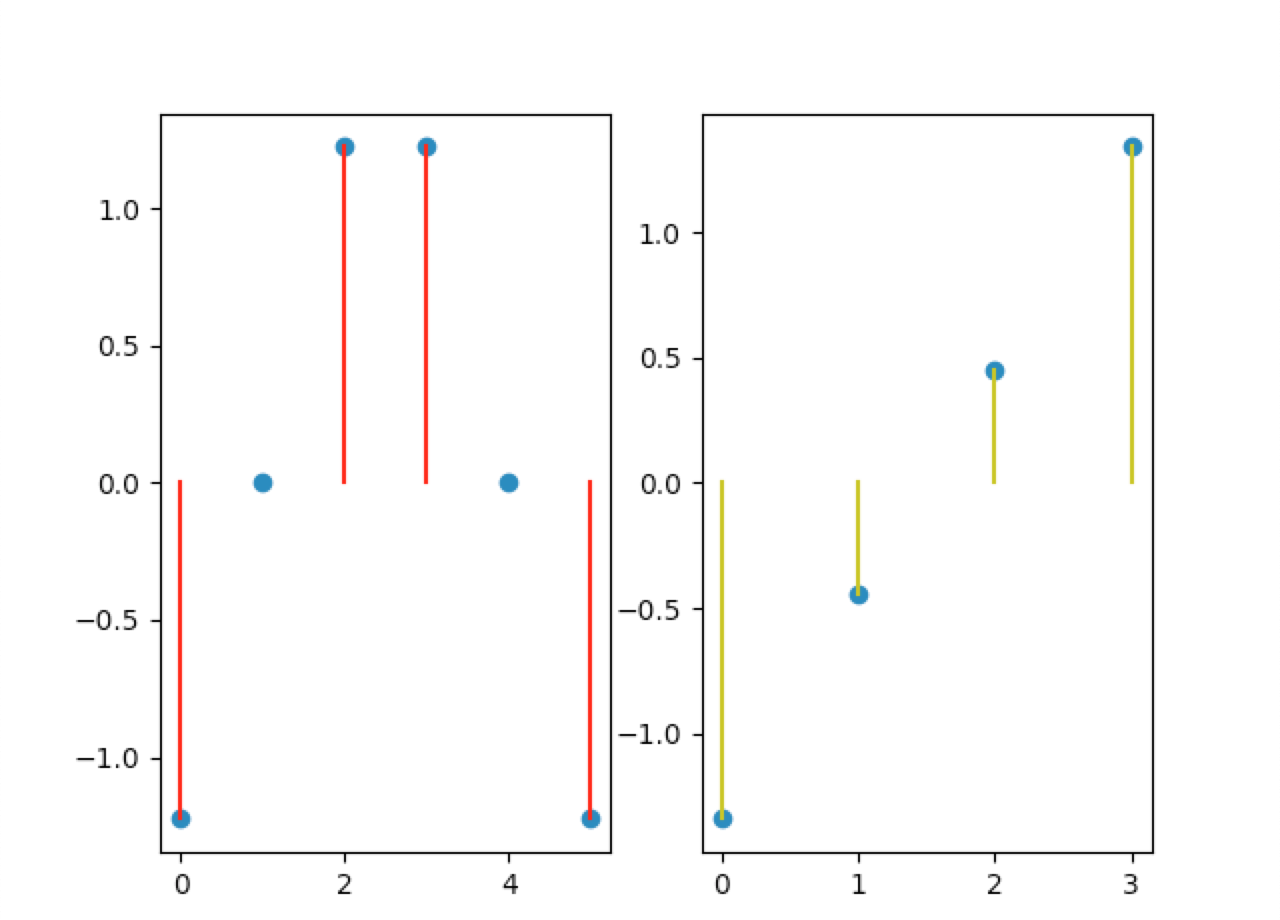
\includegraphics[width=0.5\linewidth]{figures/3b.png}
         \label{fig:3b}
     \end{figure}\\
     \part{functionC} [0, 4, 16, 36, 60, 64, 44, 16, 0]\\
     \part{functionD} [1.6431676725154982, 0.5477225575051661, -2.1908902300206643, -3.8340579025361627, 0.0, 3.8340579025361627, 2.1908902300206643, -0.5477225575051661, -1.6431676725154982]\\
     \cleardoublepage
     \question{4. Signal}{}
     \part{functionA}
     \begin{figure}[h]
         \centering
         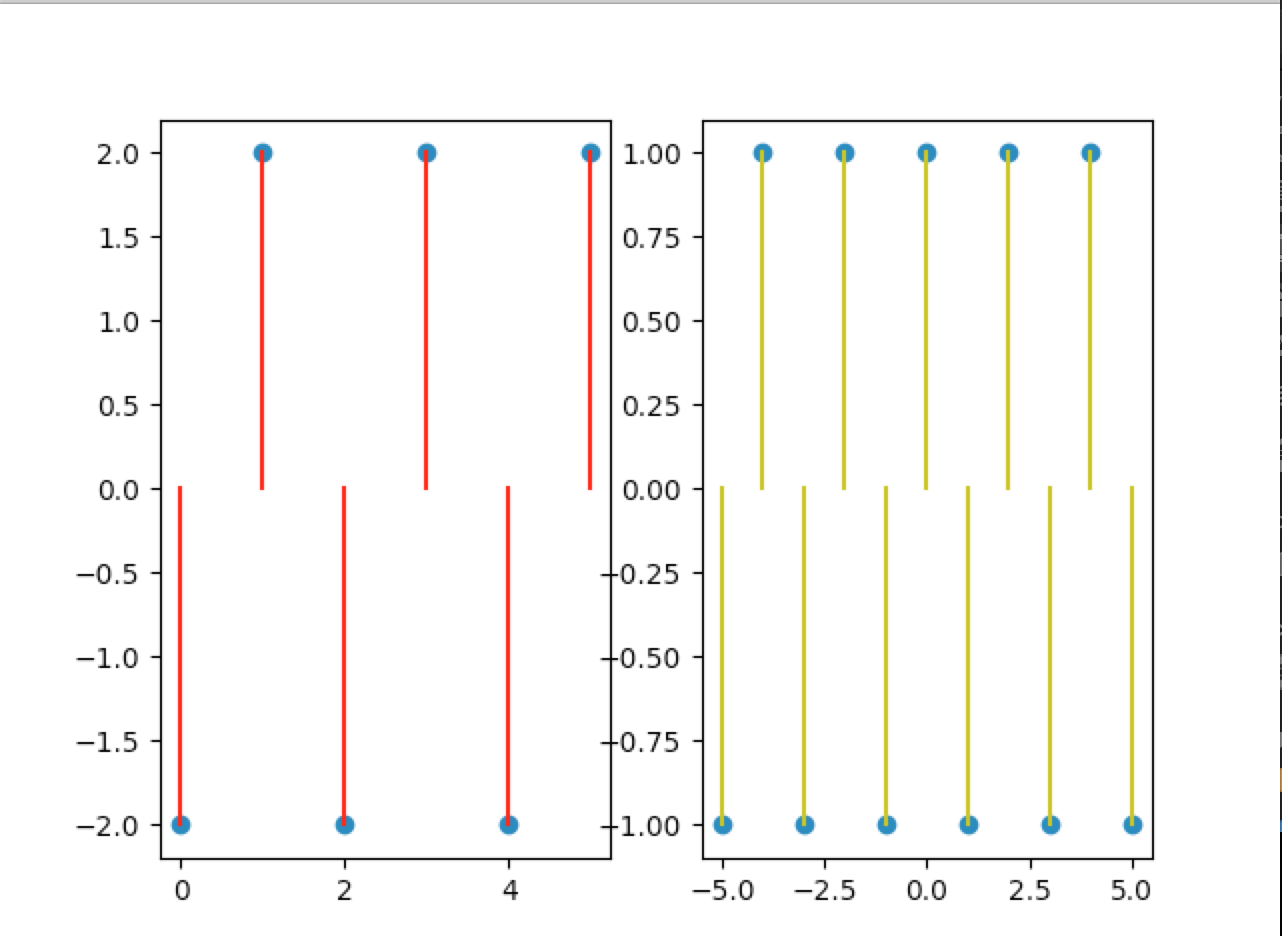
\includegraphics[width=0.5\linewidth]{figures/4a.png}
         \label{fig:4a}
     \end{figure}\\
     \part{functionB}
     \begin{figure}[h]
         \centering
         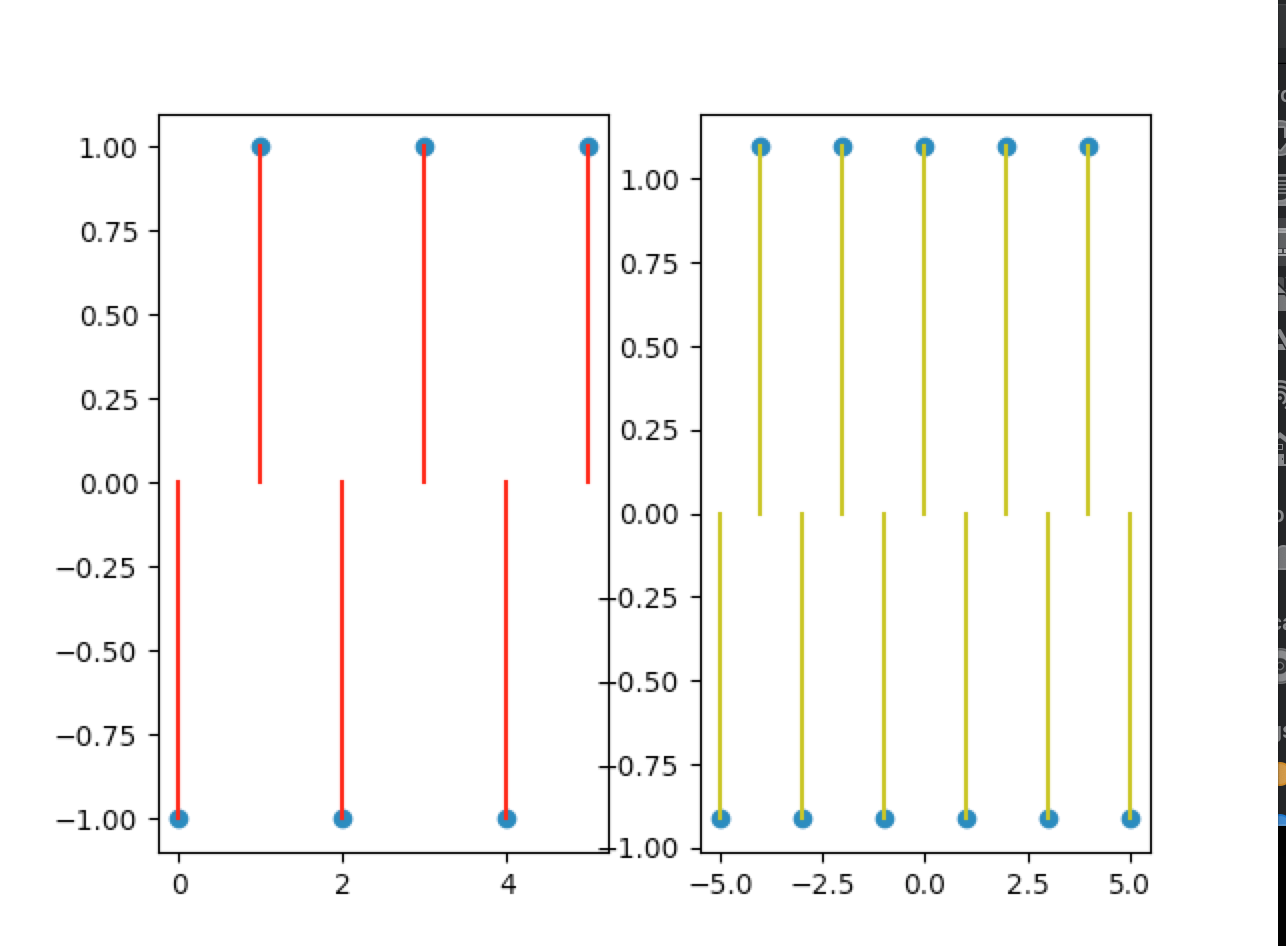
\includegraphics[width=0.5\linewidth]{figures/4b.png}
         \label{fig:4b}
     \end{figure}\\
     \part{functionC} [2, -4, 6, -8, 10, -12, 12, -12, 12, -12, 12, -10, 8, -6, 4, -2]\\
     \part{functionD} [0.9128709291752769, -2.008316044185609, 2.921186973360886, -4.016632088371218, 4.929503017546495, -6.024948132556828, 6.024948132556828, -6.024948132556828, 6.024948132556828, -6.024948132556828, 6.024948132556828, -4.929503017546495, 4.016632088371218, -2.921186973360886, 2.008316044185609, -0.9128709291752769]\\
     
	
\end{document}
